\chapter{Dark Matter Properties} \label{Dark matter properties}

As anticipated in the previous chapter, only about 31\% of the universe is composed of matter, and a mere 5\% of this is ordinary (baryonic) matter. This leaves a significant portion of the cosmos which composition and behavior cannot be explained by visible matter alone.
In this chapter, we will focus on the first experimental evidence of the existence of dark matter proposed by Zwicky in ref. \cite{Zwicky-1937} and Vera Rubin in ref. \cite{Vera-Rubin}.\\ There are many models used to describe the distribution of dark matter density profiles, like the Einasto profile, the Burkert profile (ref. \cite{Burkert_1995}) and, for us in this thesis, the most used, the Navarro-Frenk-White profile (ref. \cite{Navarro_1997}). Following, we will briefly explain the cusp-core problem (ref. \cite{Cusp-Core-Problem-Del-Popolo}), the missing satellite problem (ref. \cite{too-many-dwarf-galaxy-satellites-problem}) and some possible solutions. Finally, we will discuss the nature of dark matter as well as its interactions with baryonic matter and dark matter itself (ref. \cite{Galaxy-cluster-self-interacting-dark-matter-simulations}).

\section{Experimental Evidence for the Existence of Dark Matter}

\subsection{First Evidence by Zwicky}
One of the earliest pieces of evidence for the existence of dark matter comes from Fritz Zwicky’s 1933 observations of the Coma galaxy cluster (ref. \cite{Zwicky-1937}). This cluster is composed of approximately 800 galaxies, each with an estimated mass of about $10^9 \; M_\odot$. 

The gravitational potential energy can be expressed as
\begin{equation}\label{potential energy}
    \langle U \rangle = - \int_0 ^R \frac{G M(r)}{r} \, dm,
\end{equation}
where $M(r)$ is the mass enclosed within radius $r$. Assuming a uniform mass distribution, we can write:
\begin{equation}
    M(r) = \frac{4}{3} \pi r^3 \rho \quad \Rightarrow \quad dm = 4 \pi r^2 \rho \, dr,
\end{equation}
with $\rho$ representing the average density of the cluster. Substituting into eq. \eqref{potential energy}, we obtain:
\begin{equation}
    \langle U \rangle = - \int_0^R \frac{G \cdot \left(\frac{4}{3} \pi r^3 \rho\right)}{r} \cdot 4 \pi r^2 \rho \, dr 
    = -\frac{3}{5} \frac{G M_{\text{tot}}^2}{R},
\end{equation}
where the total mass is
\begin{equation}
    M_{\text{tot}} = \frac{4}{3} \pi R^3 \rho.
\end{equation}

Next, applying the virial theorem, $2 \langle K \rangle + \langle U \rangle = 0$, we express the average kinetic energy as:
\begin{equation}
    \langle K \rangle = \frac{1}{2} M_{\text{tot}} \sigma_v^2,
\end{equation}
where $\sigma_v$ is the velocity dispersion. Replacing the theoretical value of mass ($800 \cdot 10^9 \; M_\odot$) and solving for $\sigma_v$, we obtain:
\begin{equation}
    \sigma_v = \frac{3}{5} \sqrt{\frac{G M_{\text{tot}}}{R}} \approx 80 \; \text{km} \; \text{s}^{-1}.
\end{equation}

However, Zwicky observed a much larger value of around $1000$ km s$^{-1}$ (ref. \cite{Zwicky-1937}), significantly higher than the predicted result. Assuming the velocity dispersion measurement is correct, the total mass of the cluster must be much greater than initially estimated:
\begin{equation}
    M_{\text{tot}} = \frac{5}{3} \frac{R}{G} \sigma_v^2 \approx 1.25 \cdot 10^{14} \, M_\odot.
\end{equation}

\subsection{Rotation Curves}
Another strong piece of evidence comes from the study of galactic rotation curves, first systematically measured by Vera Rubin (ref. \cite{Vera-Rubin}). According to Newtonian dynamics and General Relativity, the rotational velocity of stars in a galaxy should decrease with increasing distance from the galactic center. However, observations reveal that these velocities tend to remain approximately constant (see fig. \ref{rotation speed of galaxy}).\\
We can assume that most of the mass of a galaxy is contained in the central part called bulge (or central bulk). Consequently, we can imagine that there is a maximum in the rotation profile almost close to the center.\\
 As a first approximation, we model the galaxy as having a constant density $\rho_0$ up to a characteristic radius $R_*$, beyond which the density drops abruptly to zero. This corresponds to a simplified top-hat density profile.
 Under this assumption, the total mass enclosed within a radius $R < R_*$ is given by:
\begin{equation}
    M(r<R) = \int_0 ^R \rho(r) d^3 x=4\pi\rho_0 \int_0 ^R r^2 dr = \frac{4}{3} \pi \rho_0 R^3,
\end{equation}
meanwhile for radii greater than $R_*$, since the density is zero by construction, the enclosed mass remains constant
\begin{equation}
    M(r>R_*) = \frac{4}{3} \pi \rho_0 R^3_*.
\end{equation}
Then, we can calculate the velocity by balancing gravitational and centrifugal forces
\begin{equation}
    v_c = \sqrt{\frac{GM (r)}{R}},
\end{equation}
that gives us two different results:
\begin{equation}
    v_c(R) \sim 
    \begin{cases}
        R & \text{for } R < R_*, \\
        R^{-\frac{1}{2}} & \text{for } R > R_*.
    \end{cases}
\end{equation}
This prediction implies that the rotation speed increases linearly in the central region (where mass grows with $R^3$), and then falls off at larger radii (since no additional mass is enclosed beyond $R_*$).
However, this theoretical profile does not match observations: rotation curves of spiral galaxies tend to flatten out at larger radii rather than decline like we can see in fig. \ref{rotation speed of galaxy} below. 

\begin{figure}[h!]
\centering
    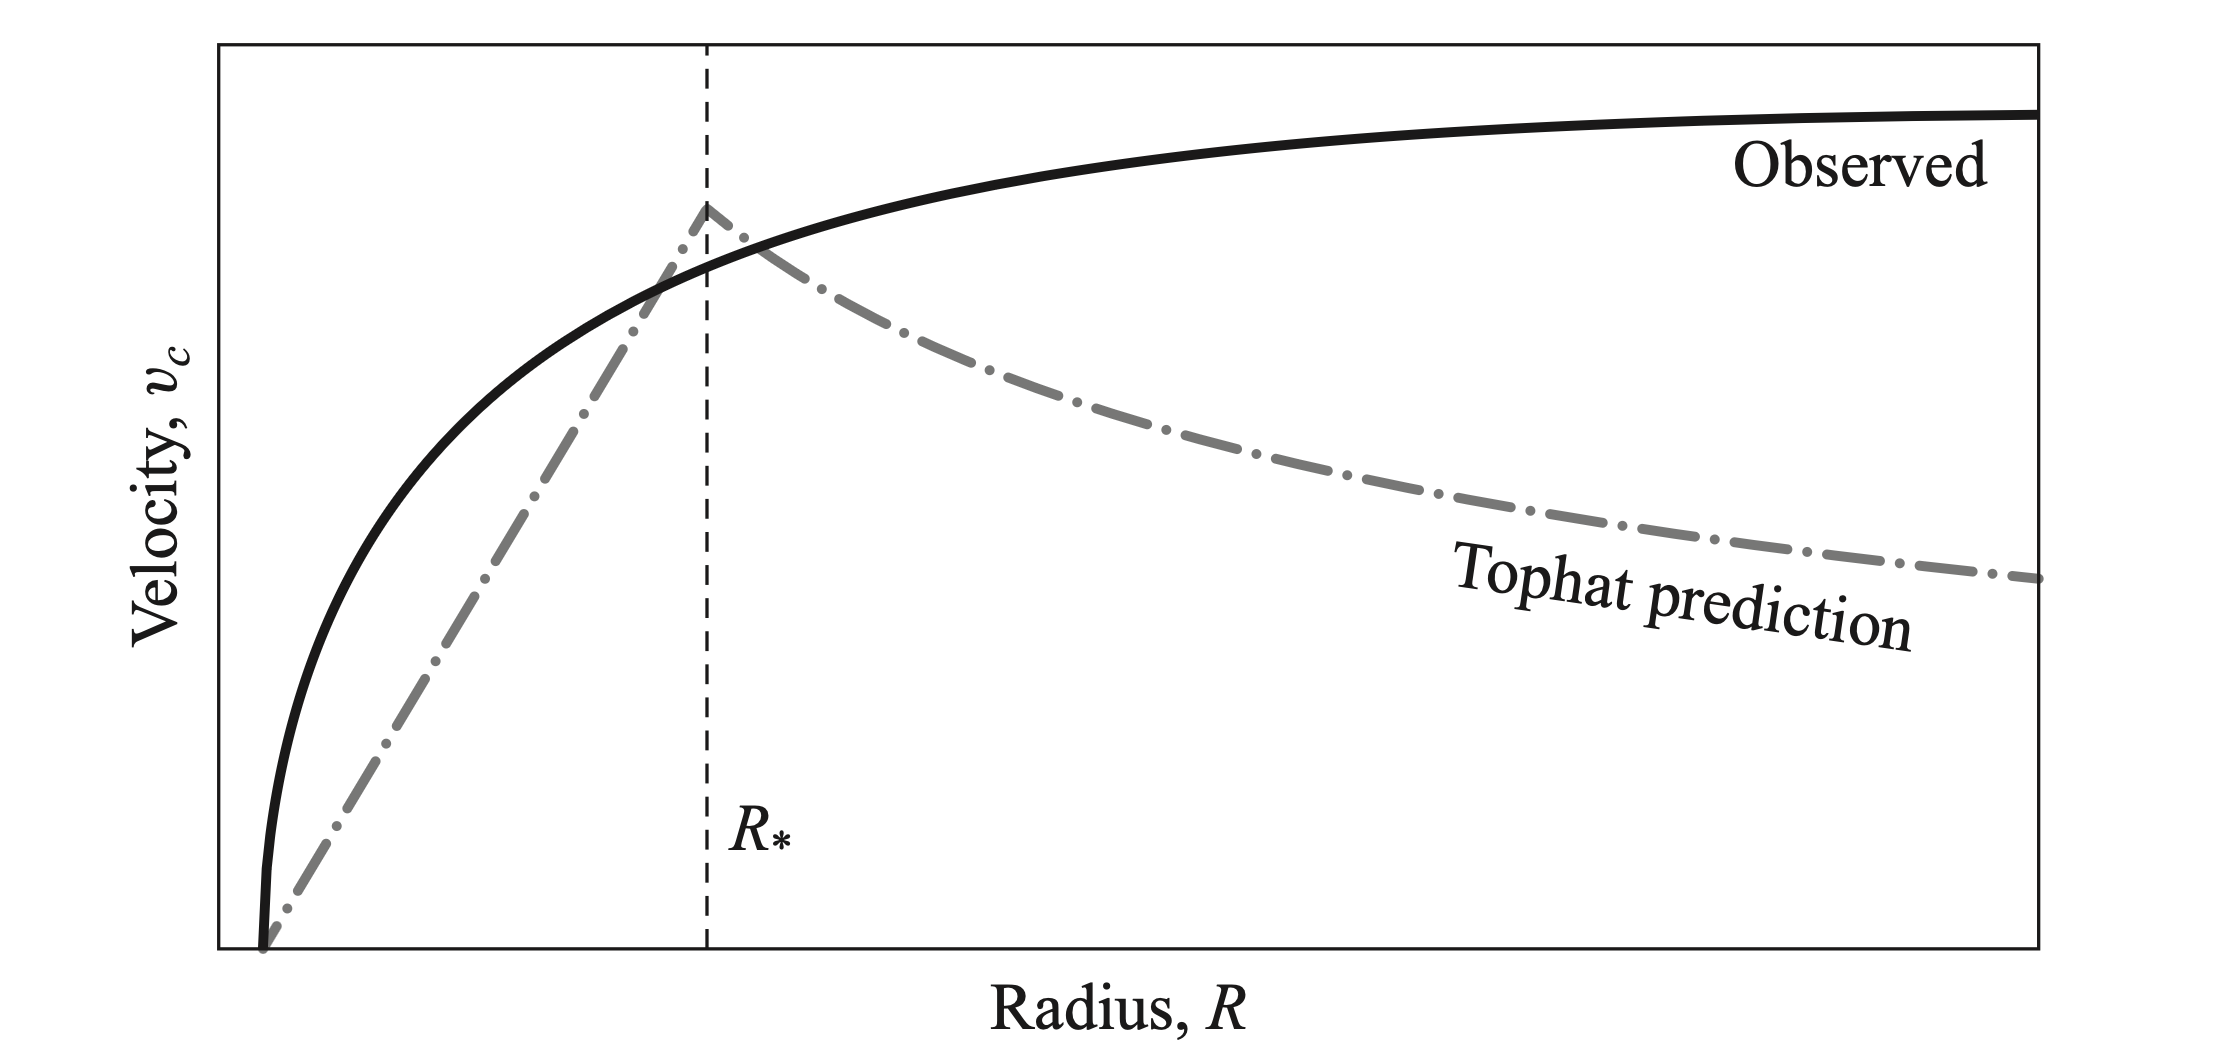
\includegraphics[width=0.65\linewidth]{Images/Chapter2/Rotation curve.png}
    \caption[Rotation curve of a galaxy]{Rotation curve of a galaxy. The dotted line represents the theoretical prediction, while the solid black line shows the observed curve. Figure 3.5 in ref. \cite{2024darkmatter}.}
\label{rotation speed of galaxy}
\end{figure}

Another important demonstration of the existence of dark matter is the anisotropies in the CMB (fluctuation power spectrum); this contains much information to determine the parameters of the standard cosmological model. In particular, as we said in Chapter \ref{Capitolo 1}, before the recombination era, the universe was a dense plasma where baryons and photons were coupled. This fluid had small oscillations called baryonic acoustic oscillations (BAO), waves of pressure that propagated in the plasma. The velocity of these perturbations is the sound speed in this fluid, indicated by $c_s^2$.\\ BAO remains as a footprint in the CMB spectrum. In figure \ref{CMB power spectrum} below, the power spectrum of the CMB is shown. Green dots are data points with their error bars; at high and low multipoles, the model is well fitted by baryons and cold dark matter, while only in a very small region is it fitted by baryons only.

\begin{figure}[h!]
\centering
    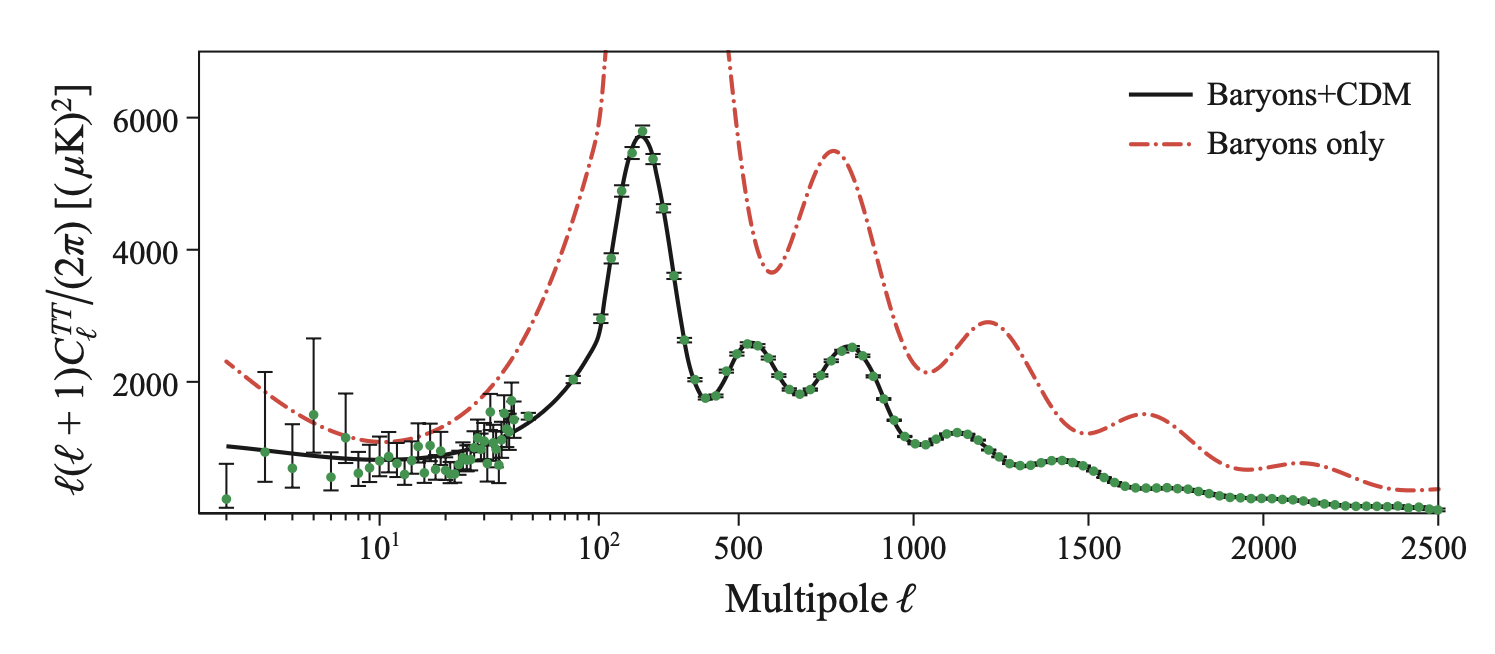
\includegraphics[width=0.7\linewidth]{Images/Chapter2/Screen dark matter libro.png}
    \caption[CMB power spectrum]{CMB power spectrum. On the $x$-axis the multipoles are reported and, on the $y$-axis, the amplitude of acoustic oscillations are reported. Figure 6.5 in ref. \cite{2024darkmatter}.}
\label{CMB power spectrum}
\end{figure}

All these discrepancies indicate a significant amount of mass is present beyond the visible component — leading to the hypothesis of dark matter halos surrounding galaxies.\\
Over the decades, many hypotheses have been proposed to explain the nature of dark matter and, more generally, the missing mass. These include:
\begin{itemize}
    \item Warm, hot and cold dark matter
    \item MACHOs (Massive Compact Halo Objects)
    \item WIMPs (Weakly Interacting Massive Particles)
    \item Modified Gravity Theories
\end{itemize}

MACHOs are "composed" by very compact objects like black holes, neutrons stars and white dwarfs. However, none of these can explain the nature of dark matter because neutron stars and white dwarfs emit electromagnetic radiation, while the number of black holes necessary to explain the entire missing mass would be too high. Furthermore, from a statistical point of view, some stars would accrete onto them and emit electromagnetic radiation (ref. \cite{Astrophysics-in-a-Nutshell}).\\
WIMPs are hypothetical particles $\chi$ with a rest mass $m_\chi$ in the range of 1–10 GeV (ref. \cite{Longair}). These particles interact very weakly with Standard Model particles. In the early Universe, it was hot enough to produce $\chi$ and $\bar\chi$ in thermal equilibrium, but when the temperature fell below $T \sim m_\chi$, annihilation reactions could no longer maintain that equilibrium. Under this temperature, the abundance froze out.\\ A typical weak scale annihilation cross section $\langle \sigma v\rangle \sim 10^{-26} \; \text{cm}^3 \; \text{s}^{-1}$ naturally yields the observed dark matter relic density; this is the so-called “WIMP miracle” (ref. \cite{2024darkmatter}).\\
Modified gravity theories include several theoretical models that attempt to modify gravity by potentially extending General Relativity; for example there are tensor-scalar theories that include $f(R)$ gravity, Brans-Dicke theory, Degenerate Higher-Order Scalar-Tensor (DHOST) or tensor-vector-scalar theories like MOND (Modified Newtonian Dynamics).\\
However, not all modified gravity models are designed to explain dark matter, in fact, MOND its relativistic extension were explicitly developed as alternatives to dark matter, aiming to reproduce galactic rotation curves without invoking unseen mass (ref. \cite{Milgrom_1983_MOND}).\\ $f(R)$ gravity try to include the effects of dark matter and dark energy into the curvature of space-time (ref. \cite{Capozziello_2006}) while Brans-Dicke and DHOST theories focus their attention on dark energy (ref. \cite{langlois2018degeneratehigherorderscalartensordhost}).\\

In the rest of the chapter, as previously mentioned, we will focus on dark matter models.

\section{Navarro-Frenk-White Dark Matter Density Profile}

In order to investigate the role of dark matter and its properties, we introduce the Navarro-Frenk-White (NFW), a universal model for fitting the slope of dark halos proposed by Julio Navarro, Carlos Frenk e Simon White during 1996 (ref. \cite{Navarro_1996}, \cite{Navarro_1997}) after simulations of dark matter. An important feature of this model is its universality: the NFW profile successfully describes dark matter halos across a wide range of masses and redshifts, making it a robust and widely adopted tool in cosmology, as demonstrated in ref. \cite{Navarro_1997}.
The Navarro-Frenk-White analytical form is the following:
\begin{equation}\label{NFW}
    \rho (r) = \rho_c(z) \frac{\delta_c}{\frac{r}{r_s} \qty (1+\frac{r}{r_s})^2}.
\end{equation}
Here $\delta_c$ is a characteristic dimensionless density, $r_s$ is the scale radius and $\rho_c(z)$ the critical density at time $z$.
Physically, $r_s$ is the radius that indicates where the profile becomes steeper.\\ From a mathematical point of view $r_s = r_{-2}$, where $r_{-2}$ denotes the radius at which the derivative of the logarithm of the density is equal to $-2$.\\
The radial profile is proportional to $r^{-1}$ at small radii and $r^{-3}$ at large radii.\\
As we can see in the following figure \ref{NFW_fit_1996}, the uniformly good fits across all masses and cosmologies provide clear evidence for the universality of the NFW profile, even in different cosmologies.

\begin{figure}[h!]
\centering
    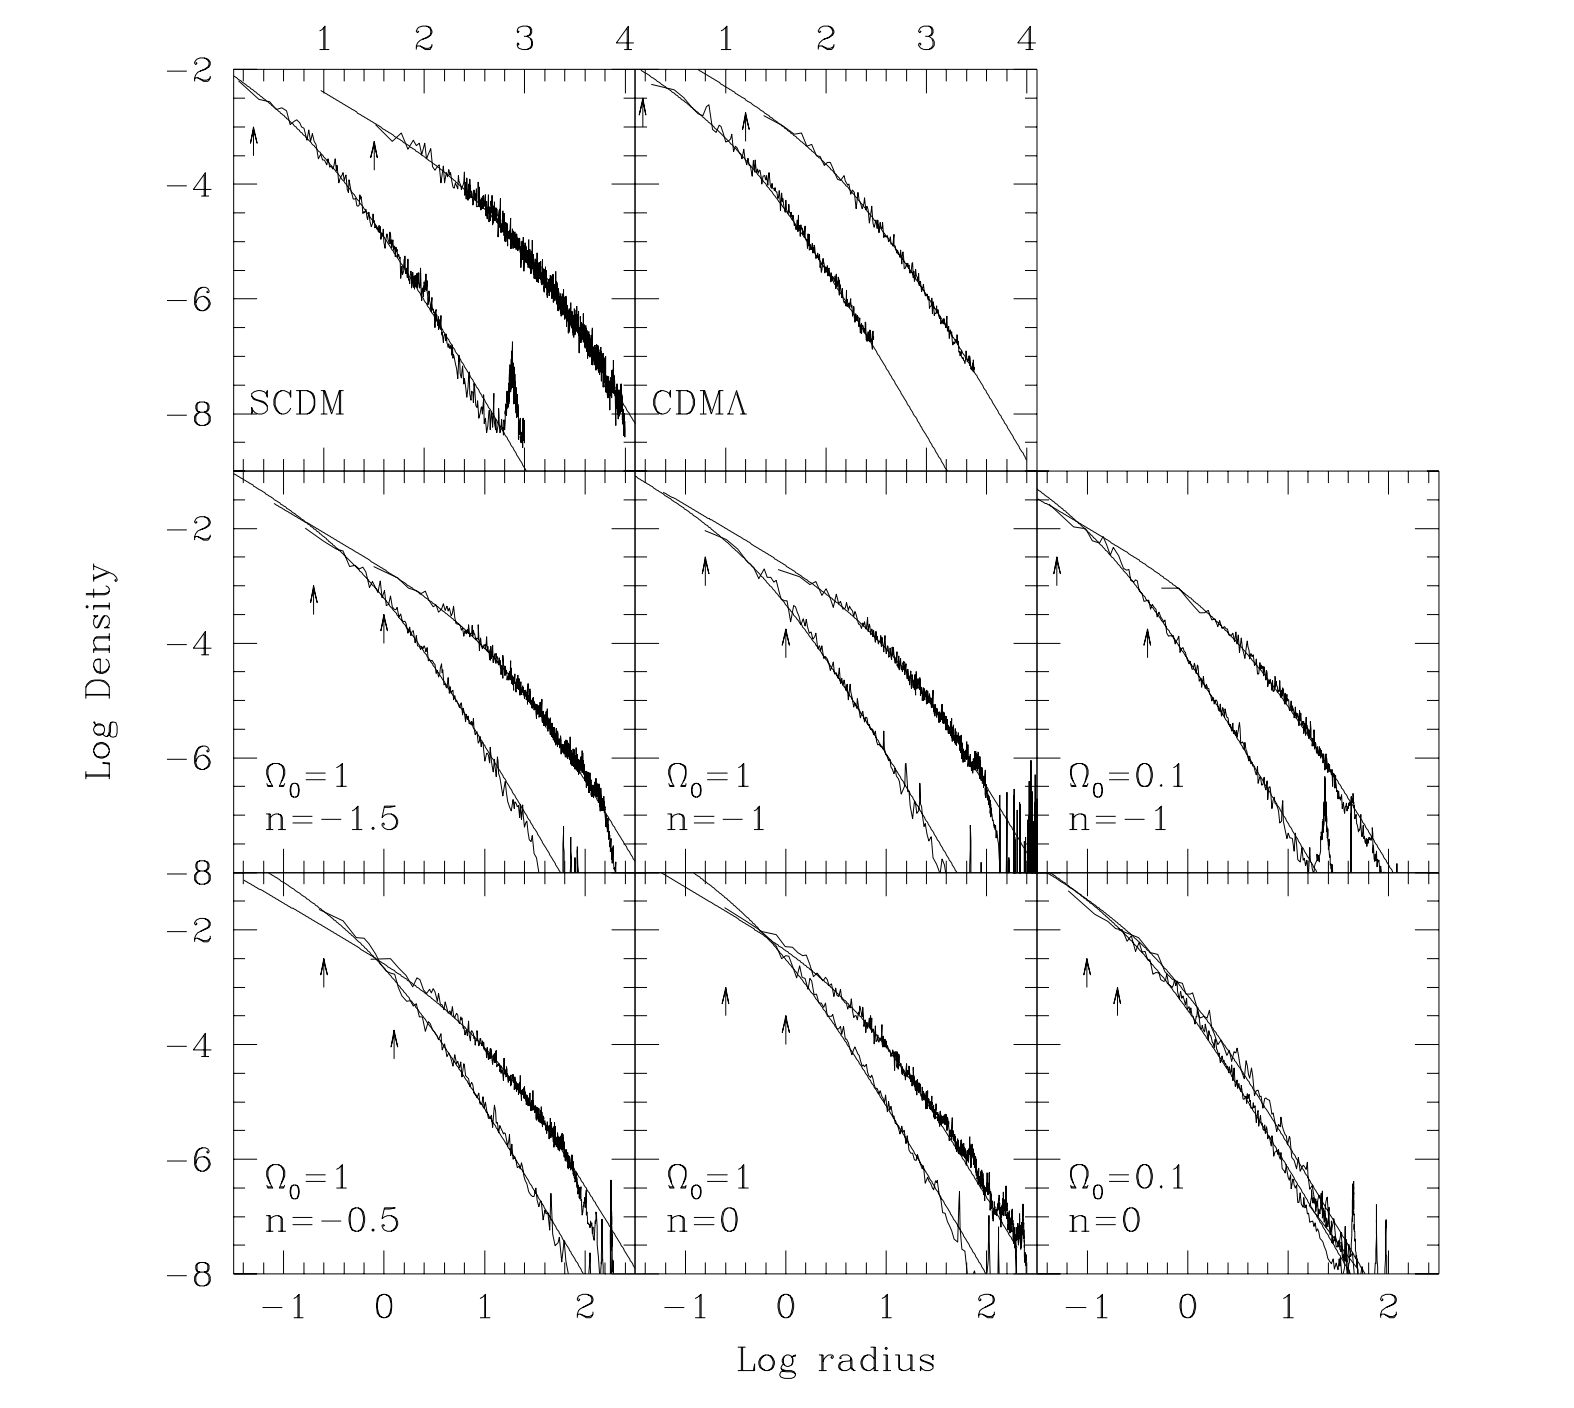
\includegraphics[width=0.68\linewidth]{Images/Chapter2/NFW_1996.png}
    \caption[Evidence for the universal NFW density profile]{Density profile of two dark matter haloes, the left-hand curve in each panel rapresent the low mass halo and the right-hand curve the massive halo. The thick jagged lines in each panel are the data obtain from simulation while the thin smooth curves are the two-parameter NFW fits. Credits \cite{Navarro_1997}.}
\label{NFW_fit_1996}
\end{figure}

It is also useful to introduce additional quantities and physical relationships, such as $r_{200}$, $M_{200}$ and the concentration $c = \frac{r_{200}}{r_s}$ (sometimes indicated with $c_{200}$). 
The radius $r_{200}$ is defined as the radius within which the average density is 200 times the critical density of the Universe. The corresponding mass $M_{200}$ is calculated as:
\begin{equation}
M_{200}=\frac{100H^2(z)r_{200}^3}{G},
\end{equation}
but remembering that the critical density is $\rho_c(z)=\frac{3H^2(z)}{8\pi G}$ and combining these two equations it's possible to find
\begin{equation}
    M_{200} = \frac{4}{3} \pi r_{200}^3 \cdot 200 \rho_c.
\end{equation}
The characteristic density is related to the concentration $c$ through the following formula (ref. \cite{Navarro_1997})
\begin{equation}
    \delta_c = \frac{200}{3} \frac{c^3}{[\ln(1+c)-c/(1+c)]},
\end{equation}
then, this one can be expressed as:
\begin{equation}
    \rho_s = \rho_c(z) \cdot \delta_c = \frac{M_{200}}{4\pi r_s^3 \qty[\ln(1+c)-c/(1+c)]}.
\end{equation}

This model provides a mass density profile for galaxy clusters and their dark matter halos.
However, there are some differences between simulations and observations. For example, the Navarro-Frenk-White model is affected by the so-called cusp problem, according to which the dark matter density profile is expected to rise steeply toward a peak near the central region—where most of the matter is concentrated—and then drop off rapidly. However, this trend is not observed experimentally.
Due to this singularity, it's also possible to define the generalized Navarro-Frenk-White (see e.g. ref. \cite{Wyithe_gNFW_2001}), also called gNFW hereafter, introducing $\gamma$:
\begin{equation}\label{gNFW}
    \rho (r) = \frac{\rho_s}{\left(\frac{r}{r_s}\right)^\gamma \left(1+\frac{r}{r_s}\right)^{3-\gamma}},
\end{equation}
where $0<\gamma<2$ (note that by setting $\gamma = 1$, we obtain the standard Navarro-Frenk-White density profile) and $\rho_s$ is the scale density defined as follows
\begin{equation}
    \rho_s = \qty(\frac{r_{200}}{r_s})^{\gamma-3} \frac{M_{200}(3-\gamma)}{4\pi r_s^3 \, {}_2F_1\qty(3-\gamma, 3-\gamma; 4-\gamma; -\frac{r_{200}}{r_s})},
\end{equation}
where $_2F_1$ is an hypergeometric function.\\
In this model, an arbitrary law shaped the central cusp with $r^{-\gamma}$ while, out of the central region, it falls off as $r^{-3}$ (ref. \cite{Wyithe_gNFW_2001}).\\
Inside a galaxy cluster, most of the mass is contained in the dark halo and offers us a perfect natural laboratory to test and study dark matter models.\\
\begin{figure}[h!]
\centering
    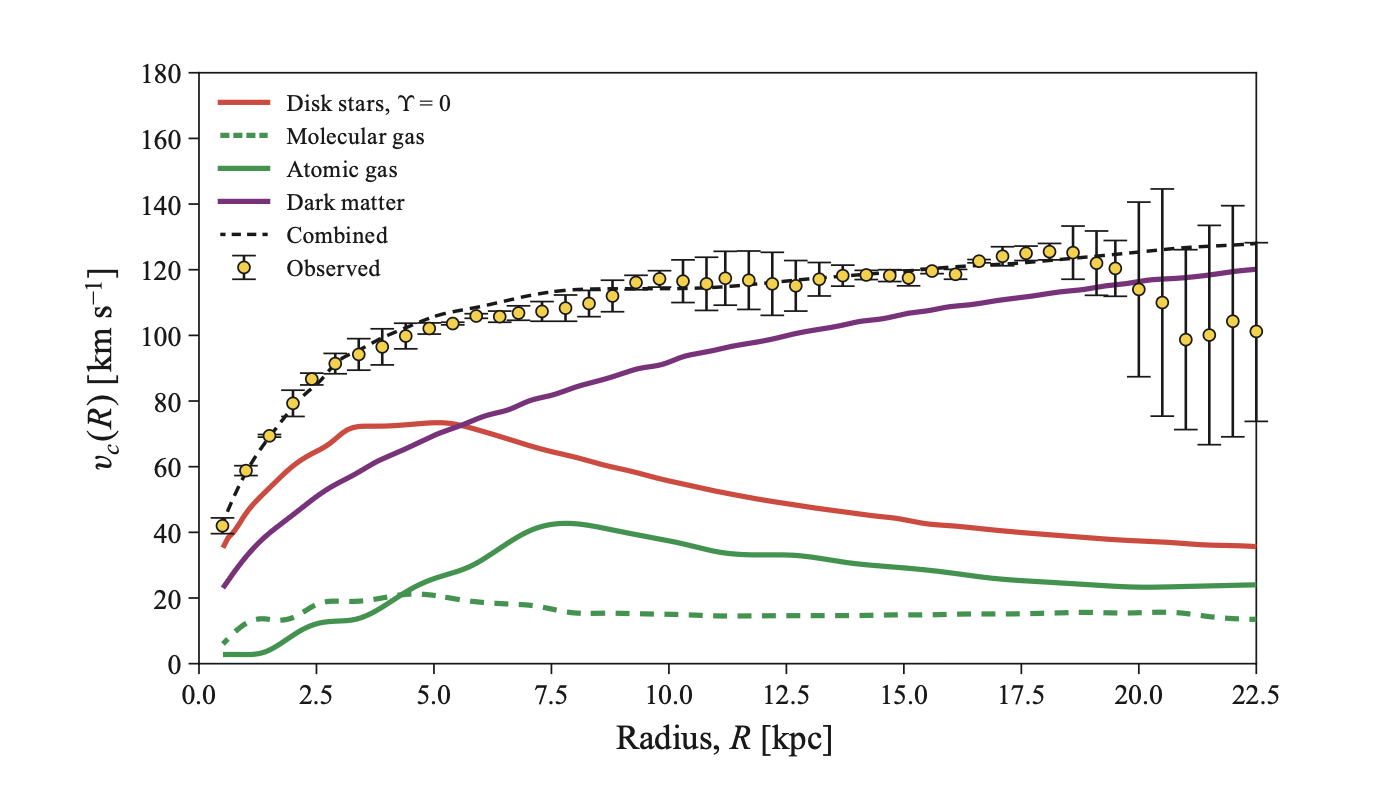
\includegraphics[width=0.682\linewidth]{Images/Chapter2/Rotation curve M33.png}
    \caption[Rotation curve of M33]{According to the figure 3.7 in ref. \cite{2024darkmatter} this is the best fit with the NFW model for the rotational curve of M33 (Triangulum Galaxy).}
\label{rotation speed of galaxy}
\end{figure}
\noindent Due to the strong dependence of $\rho(r)$ on the nature of dark matter, determining the value of $\gamma$ is a crucial step in improving our understanding of dark matter. In particular, values of $\gamma < 1$ may indicate the presence of fuzzy, decaying, or self-interacting dark matter, while higher values ($\gamma > 1$) can result from mass accretion processes, as discussed in ref. \cite{CLASH-VLT:-The-Inner-Slope-of-the-MACS-J1206.2-0847-Dark-Matter-Density-Profile}.\\

There are also several dark matter profiles such as the Einasto profile or Burkert profile whose mathematical expressions are, respectively, the following:
\begin{equation}
    \rho(r) = \rho_s \text{exp} \qty{-2m\qty[\qty(\frac{r}{r_s})^{\frac{1}{m}}-1]} \qquad \rho (r) = \frac{\rho_s}{\qty(1+\frac{r}{r_s}) \qty[1 + \qty(\frac{r}{r_s})^2]}.
\end{equation}
with $m \in \mathbb{N}$ in the Einasto profile. While the NFW model exhibits a cusp, diverging at small radii, the Einasto and Burkert profiles flatten to a constant value for $r \rightarrow 0$.
\begin{figure}[h!]
    \centering
    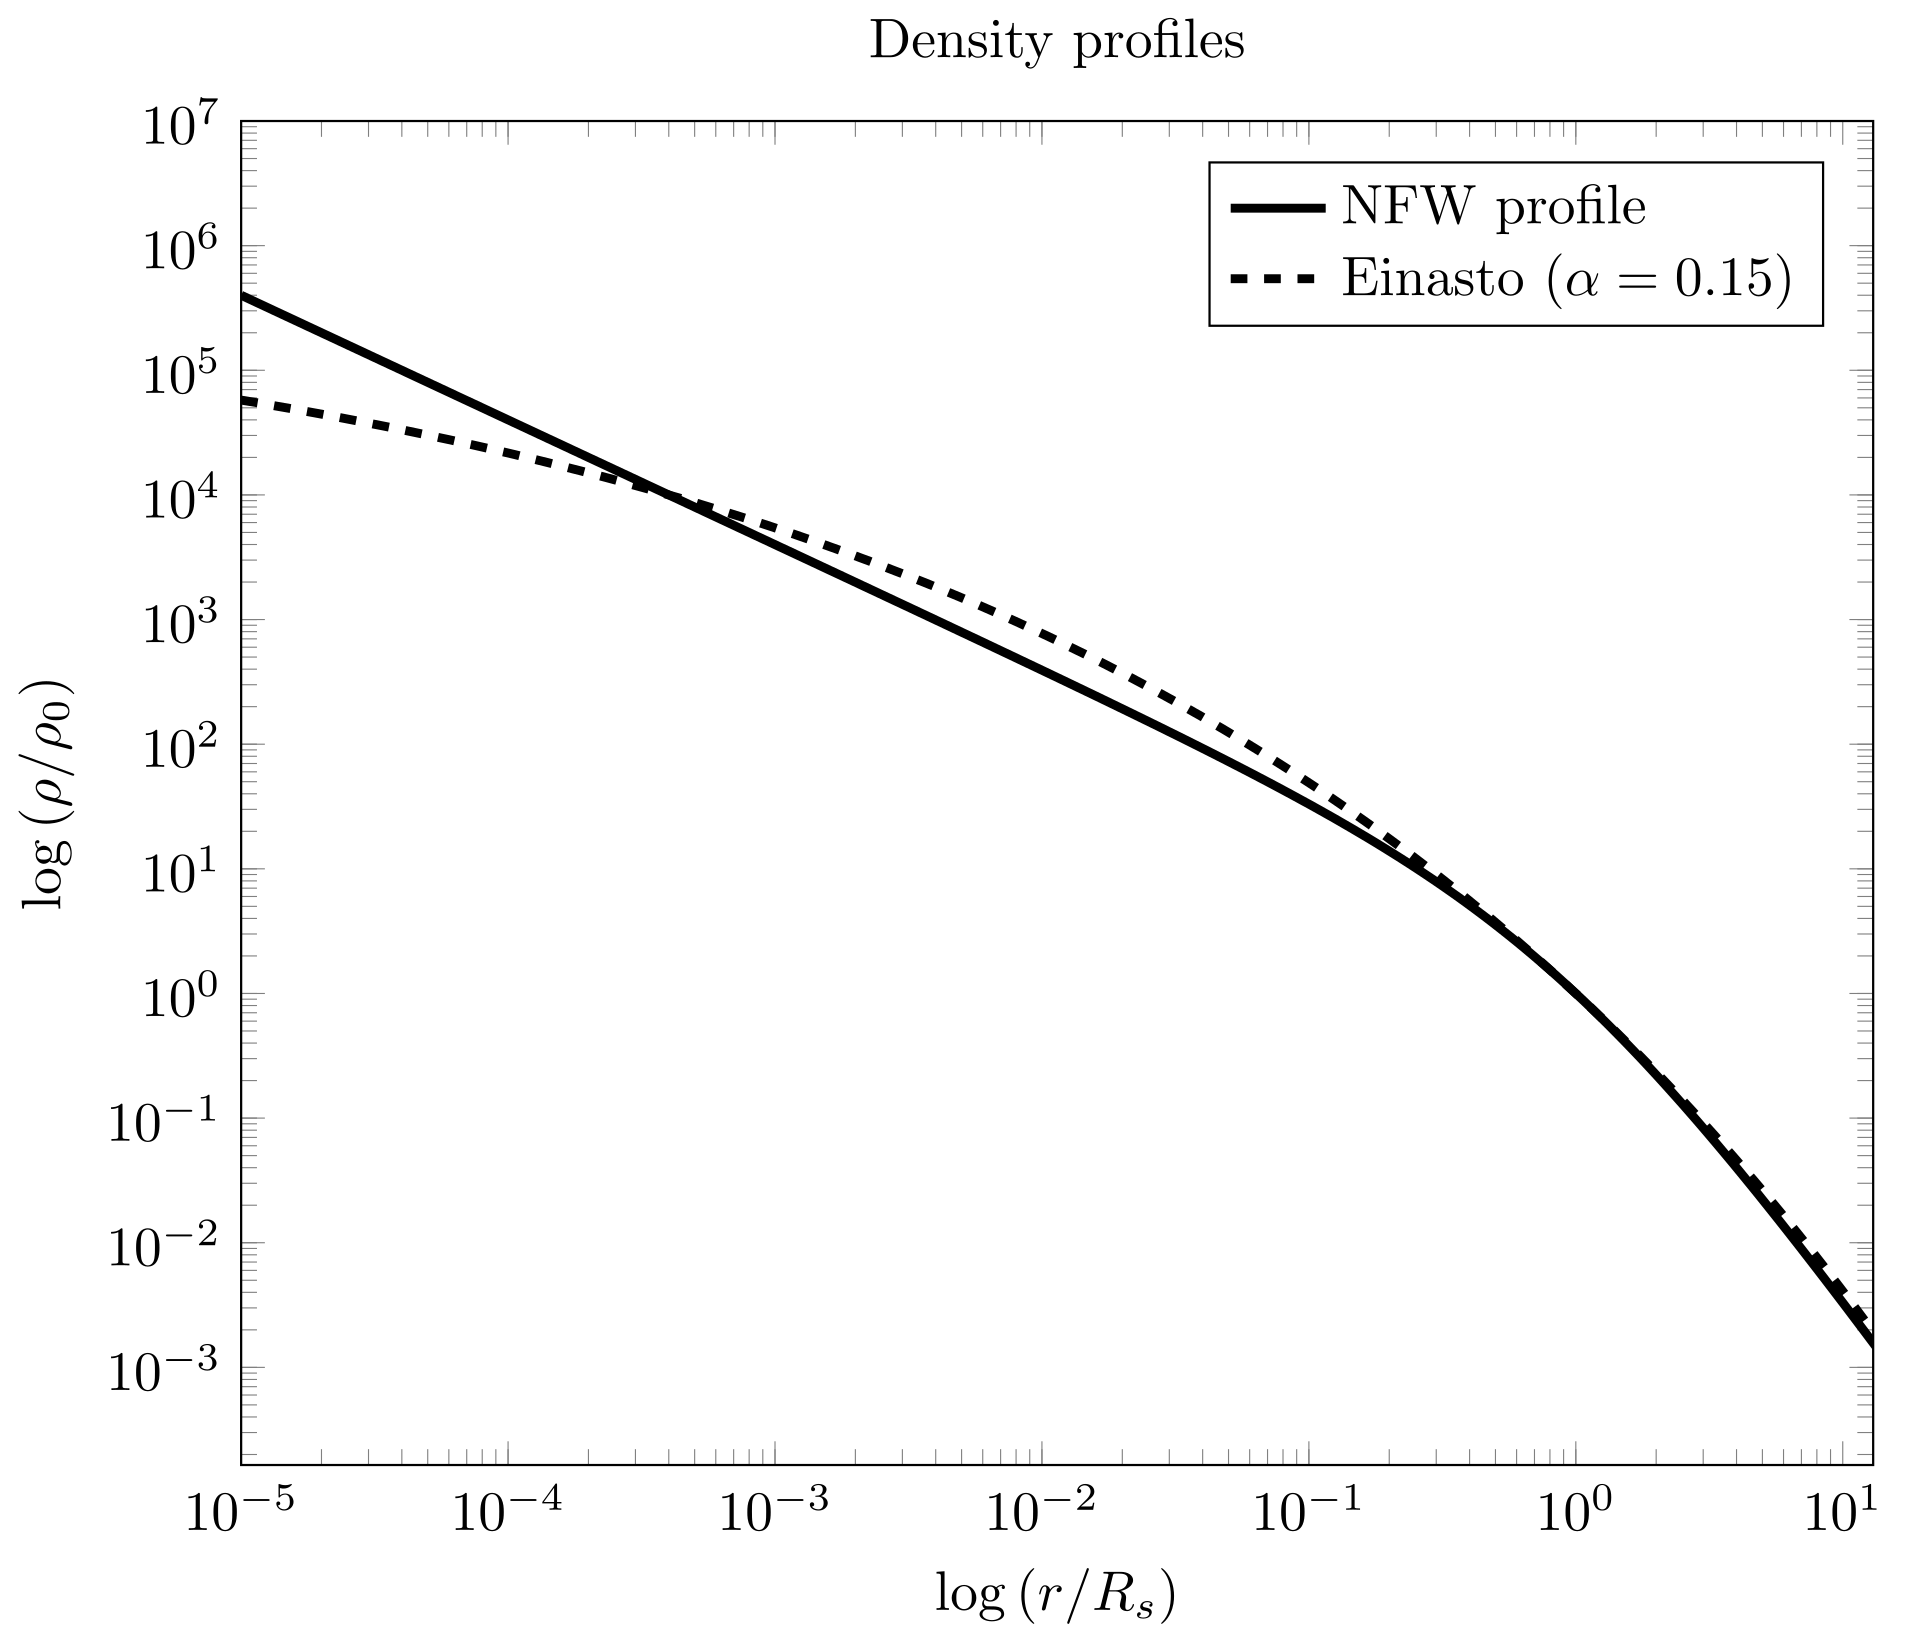
\includegraphics[width=0.4925\linewidth]{Images/Chapter2/Comparison_of_NFW_and_Einasto_profiles.svg.png}
    \caption[Comparison between NFW and Einasto profiles]{Comparison between NFW and Einasto profiles in log scale. Credits \cite{wikiNFWprofile}.}
\label{NFW and Einasto profile}
\end{figure}

\section{Cusp-core problem}
The cusp-core problem (also called the CC problem) is that some galactic rotation curves are better described by models that do not have a cusp, such as the isothermal density profile. This is in contrast to the N-body simulation which, like the NFW model, predicts the formation of a cusp profile.
The first attempts to solve the CC problem involved looking for statistical errors with observation or simulation limits. Other possible explanations include the baryonic effect (gas and stars for example) in the dark matter profile or cosmological solutions that change the $\Lambda$CDM model according to ref. \cite{Cusp-Core-Problem-Del-Popolo}.

\subsection{Baryonic solution}
The baryonic solution includes three possible effects: Supernovae Feedback Flattening (SNFF), Dynamical Friction from Baryonic Clumps (DFBC) and Mass-dependent density profiles.\\
The SNFF mechanism is very similar to AGN feedback, with the difference that the latter only occurs if the galaxy has an active black hole at its center, while SNFF can also occur in smaller galaxies. For this reason, we will focus on SNFF.
In the first one, supernovae explosions transfer energy to gas that change the gravitational potential. This perturbation is "sensed" by dark matter expanding its distribution, forming a core. This mechanism works better in small galaxies (dwarf galaxies). However, a single supernova is not enough. For this model to be valid, repeated supernova explosions are needed.
Instead, the baryonic clumps fall toward the center of the gravitational potential and transfer energy due to friction with the dark matter. This leads to a redistribution of dark matter that flattens the cusp.\\ 
Another criticism of the SNFF model is the need for too high a star formation rate. So only for $M > 10^6 \; M_\odot$ there is a good approximation between the stellar mass and the profile slope.\\ The physical mechanism of DFBC can be divided into several phases: the linear phase where proto-galactic structures composed of dark matter and refusals of gas are formed. In the second phase, dark matter gravitationally collapses, forming potential wells that attract baryonic matter. The falling unstable gas fragments into dense clumps of gas, forming disks. When the surface density of the disk exceeds a critical threshold, the disk becomes particularly unstable and fragments into clumps in Jeans equilibrium capable of reaching considerable dimensions and masses. A small part of the gas in the clumps forms stars. Due to dynamical friction, energy and angular momentum are transferred to the dark matter. This process compensates for the adiabatic contraction of the dark matter. At this point (with a redshift $z\sim2$) the SNFF model can be resumed, which destroys the smaller clumps. This model works fine within $M < 10^6 \; M_\odot$ where SNFF fails. The main problem with this model is the presence of bulges or swellings, which are in fact capable of reforming the cusps.\\

Last baryonic solution is the mass-dependent density profiles. Using another form of generalized NFW (gNFW) written as follows (ref. \cite{Cusp-Core-Problem-Del-Popolo}):
\begin{equation}
    \rho(r) = \frac{\rho_s}{\qty(\frac{r}{r_s})^\gamma \qty[1+ \qty(\frac{r}{r_s})^\alpha]^{(\beta-\gamma)/\alpha}},
\end{equation}
where 
\begin{align}
\alpha &= 2.94 - \log_{10} \left[ (10X + 2.33)^{-1.08} + (10X + 2.33)^{2.29} \right] \nonumber \\
\beta  &= 4.23 + 1.34X + 0.26X^{2} \\
\gamma &= -0.06 + \log_{10} \left[ (10X + 2.56)^{-0.68} + (10X + 2.56) \right], \nonumber
\end{align}
and $X = \frac{M_*}{M_{\text{halo}}}.$\footnote{Note that with $(\alpha, \beta, \gamma) = (1,3,1)$ we obtain again the NFW.}\\ The idea is to make this profile dependent on a specific mass ratio $X$. The physical meaning of the parameters is as follows: $\gamma$ indicates the internal slope, $\beta$ indicates the external slope, and $\alpha$ indicates the transition between the internal and external zone. With this dependence by mass of halo, simulation (conducted with stellar and gas mass) can fit the density profile to find the best value for these three parameters in function of mass.


\subsection{Cosmological solution}

On the contrary, cosmological solutions propose to radically modify the standard cosmological model. To do this, a different type of dark matter is proposed: Warm Dark Matter (WDM) and Self Interacting Dark Matter (SIDM).

\subsubsection{Warm Dark Matter}

The warm dark matter is a deviation from the standard cold dark matter used in the $\Lambda$CDM model. Due to the decrease in speed, in function of time, DM should be more important in the past, dampening the formation of structure on small scales. This is very similar to the dynamical friction from baryonic clumps that heat the dark matter. Thanks to higher velocity, the density profile is flattened. However, also WDM is not a perfect solution; in order to produce sufficiently large cores ($\sim$ 1 kpc) and alleviate the cusp-core problem, Warm Dark Matter would require a very low particle mass ($\sim$ 0.1 keV). However, such a low mass is incompatible with the formation of large-scale structures, which instead demand higher masses ($\sim$ 1–2 keV). On the other hand, WDM particles with masses in that range produce only very small cores ($\sim$ 10–20 pc), which are too small to solve the cusp-core problem. Therefore, a single WDM particle mass cannot simultaneously account for both the observed cored density profiles in dwarf galaxies and the successful formation of large-scale structure, highlighting a fundamental tension within the WDM scenario.

\subsubsection{Self Interacting Dark Matter}

The last type of dark matter proposed is self-interacting dark matter (SIDM), analyzed in ref. \cite{Galaxy-cluster-self-interacting-dark-matter-simulations}.
In this alternative model, dark matter particles interact not only through gravity but also through collisions. This is in contrast with the $\Lambda$CDM framework, which treats dark matter as perfectly collisionless.\
This type of dark matter was proposed to resolve and mitigate some discrepancies between astrophysical observations and $\Lambda$CDM simulations.\\

However, this kind of matter is not relativistic, which is why it is very different from the warm dark matter that we discussed earlier. While SIDM is still consistent with observations on large scales, many differences appear on small scales (clusters and substructures), where collisions between dark matter particles can modify the distribution of mass (ref. \cite{SIDM_2000_Spergerl}).
This contribution on the smallest scales is the key to understanding why SIDM could resolve the cusp-core problem.
Self-interaction can flatten the density profile in the core region because collisions between particles distribute energy outwards, forming a blunt core.
There is another problem that SIDM can explain: many simulations show subhalos much less dense than those observed, with a gravitational lensing signal much smaller than that observed experimentally. In the SIDM model, it is possible to form a core collapse after an initial phase of formation. When halos are initially very concentrated, the interactions can increase the concentration and density; furthermore, the densities can even exceed those predicted by the $\Lambda$CDM model. Thanks to this phenomenon, also described in the literature, SIDM is capable of describing some excess compactness observed in certain cluster substructures compared to standard $\Lambda$CDM simulations.\\

The interaction cross section identifies the probability of collision between two particles. In the $\Lambda$CDM model, this value is almost zero, but this is not the case in the SIDM model; in particular, from galaxy clusters, it is possible to find an upper limit $\sigma/m \sim 0.19 \; \text{cm}^2/\text{g}$ (ref. \cite{SIDM_cross_section_upper_limit}).
A value so small indicates a very weak interaction, contradicting what has been said so far. To solve this, many models introduce a velocity-dependent cross section. In other words, collisions between dark matter particles are frequent in systems with low relative velocities (dwarf galaxies) and rare in systems with high relative velocities (clusters).\\

In particular, in ref. 
\cite{Galaxy-cluster-self-interacting-dark-matter-simulations}, two types of SIDM are well described: frequent SIDM (fSIDM) and rare SIDM (rSIDM).
In the first one, interactions are more frequent with small angles of scattering between particles; in contrast, rSIDM describes rare, large, and isotropic scattering angles.\\

Simulations can be conducted in different regimes: only with DM (ODM) or with full physics (dark matter and baryonic matter), also called FP.
In both cases, fSIDM and rSIDM produce density profiles with flattened cores, perfectly as expected by SIDM theory. However, in the FP regime, simulated clusters show a higher central density with respect to the collisionless case. This indicates that, with baryonic physics, the DM auto interaction increases the concentration of matter in the center. 

Also the abundance of substructure in clusters is affected by changes; in fact, in DMO simulations, a strong suppression of the number of subhalos inside the cluster (probably destroyed by DM-DM collisions) is demonstrated in comparison to the collisionless model. However, when baryonic matter is included, this suppression is attenuated because self-interactions tend to push the DM outwards but stars and gas mitigate the overall mass loss and consequently the probability that the subhalo will be destroyed.\\ This is even more evident between rSIDM and fSIDM because: in rSIDM collisions are few but strong, this leaves more time for the halo to relax and the mass loss is moderate. In fSIDM collisions are frequent with small angle and the cumulative effect is very similar to a viscous brake that pushes away dark matter making the sub-halo deficit higher. 

Although self-interacting dark matter appears to resolve many inconsistencies, there are still many unresolved questions. For example, it is very difficult to reconcile an interaction cross section that, on one hand, is high enough to solve the cusp-core problem, but on the other hand, must remain very weak.
It is also difficult to perform these simulations by separating the contributions of self-interacting dark matter from those due to baryonic physics, because the latter can mask the phenomena we attribute to dark matter.
Even current technology has limitations: algorithms would have to scale down to the mean free path of dark matter particles, and this represents a limit for our computing power.


\section{Missing satellite problem}

The missing satellite problem (or MSP) is another challenge. This problem concerns the discrepancy between the number of subhalos predicted by cosmological simulations (according to $\Lambda$CDM model approximately 100 satellites are planned for Milky Way in ref. \cite{There_is_No_Missing_Satellites_Problem}) of only dark matter and the satellite galaxies observed. In particular, observations detected many fewer satellites than expected from simulation in DM regime, for example, only 10 for our galaxy (e.g. ref. \cite{There_is_No_Missing_Satellites_Problem}). This leads us to better understand the role of baryonic matter inside galaxies.
A hydrodynamical cosmological simulation was used in ref. \cite{too-many-dwarf-galaxy-satellites-problem}, covering a simulated universe box of 51.7 Mpc and using dark matter particles with a mass of $4.5 \cdot 10^5 \; M_\odot$. In the simulation, galaxies similar to M83 were modeled, meaning galaxies with a baryonic mass approximately equal to that of M83. To do this, halos with masses between $0.6$ and $1 \cdot 10^{11} \; M_\odot$ were selected (M83 has a mass of about $0.7 \cdot 10^{11} \; M_\odot$). Non-isolated galaxies were excluded, meaning galaxies with a massive neighbor within 700 kpc. This allowed the identification of 146 galaxies similar to M83 (M83 analogs).
To compare them with observations, these galaxies were placed at the same distance as M83 (4.9 Mpc) and randomly distributed in the simulated sky. All subhalos (candidate satellites) within 330 kpc of projected distance and 350 kpc along the line of sight were collected. A central region was then excluded to simulate the area occupied by the main galaxy, where the high brightness makes it difficult to detect satellites. At this point, a satellite luminosity function can be built — in other words, the number of satellites in each luminosity bin.
What was found is that 13 satellites of M83 are confirmed while of all 146 simulated analogues, 3 have no satellites brighter than $M_V = -10$ ($V$-band absolute magnitude) and 2 have only one. Most have several, but in total fewer than those actually observed for M83. In conclusion, the tension at faint end ($-14 \leq M_V \leq -12$) is $> 3\sigma$. So the discrepancy is particularly significant at low luminosities.
These results indicate an opposite problem; there are too many satellites in M83, and this is a message that $\Lambda$CDM model doesn't estimate yet the abundances of dwarf galaxies.\\

Another possibility to explain the MSP is the interaction between dark matter and baryonic matter. Like we have seen in this chapter, many past models only use dark matter, but more recent studies have demonstrated that baryonic phenomena can drastically modify the surrounding environment. In fact, this is the main idea in ref. \cite{A_BARYONIC_SOLUTION_TO_THE_MISSING_SATELLITES_PROBLEM} where Milky Way satellites are studied; in particular, the role of feedback from supernovae and tidal interaction with the galactic disk.\\ The issue arises when comparing the predicted properties (density) of these subhalos based on simulations to the observed properties of dwarf galaxies based on observations.\\ 
In the article, public catalog of subhalos of the Via Lactea II simulation is used, considering, for each subhalo, the maximum velocity at infall time $v_{\text{infall}}$ (or, in other words, the maximum of the rotation curve before entering into the main halo), the mass into 1 kpc at $z=0$ indicated with $M_{<1\text{kpc}}(z=0)$ and the orbit.
Due to the absence of baryonic matter in simulations, authors apply corrections to consider baryonic effects mentioned above \footnote{Via Lactea II only consider dark matter simulations.}.\\
This correction is applied to all subhalos with $v_{\text{infall}}<50\;\text{km}\;\text{s}^{-1}$ (it is not applied to more massive, Magellanic-like subhalos). For low-mass subhalos with $v_{\text{infall}} < 30 \; \text{km} \; \text{s}^{-1}$, the correction mimics gas loss due to UV heating/stripping and the enhanced tidal mass loss caused by the host’s baryonic disk. For more massive subhalos with $v_{\text{infall}} > 30 \; \text{km} \; \text{s}^{-1}$, the correction also accounts for the supernova-feedback-induced flattening of the central dark-matter profile, which makes these satellites more susceptible to tides.\\ When assessing complete disruption, we adopt two thresholds: for subhalos with $v_{\text{infall}} > 30 \; \text{km} \; \text{s}^{-1}$ we consider them destroyed if they have lost $>$ 90\;\% of their mass and have pericentric passages within 20 kpc; for subhalos with $v_{\text{infall}} < 30 \; \text{km} \; \text{s}^{-1}$ we consider them fully stripped if they have lost $>$ 97\;\% of their mass since infall.\\

In ref. \cite{There_is_No_Missing_Satellites_Problem}, another type of solution is proposed. This time, the focus is on the observational completeness; in fact, only a small part of our galaxy is observed in a very detailed way.
Introducing an observational completeness correction factor, defined as the integration of tridimensional density of all satellites over all virial volume divided by the volume really observed by the survey (ref. \cite{The_Luminosity_Function_of_the_Milky_Way_Satellites_2008}, \cite{THE_INVISIBLES:_A_DETECTION_ALGORITHM_TO_TRACE_THE_FAINTEST_MILKY_WAY_SATELLITES_2008}), the entire number of satellites deeply changes. The assumption of various profiles influences the correction. In a model with a more concentrated profile, such as NFW, corrections are smaller than those produced by strong tidal stripping due to the presence of a baryonic disk.\\ Thanks to this correction, we obtain a minimum number of satellites that matches the CDM predictions and, like other studies cited above, even poses the related problem known as the "too many satellites problem".